\chapter{Introduction}
\label{chap:intro}

Navigation systems assist the
process of localizing, planning and following a specific route 
where localization refers to identify one's position in space.
The location information is firstly used by the navigation 
system to identify the current position on the map and 
secondly to guide the movement from one point to the other. 
A precise localization is therefore 
very important and is required for an effective 
performance of a navigation system.
The navigation systems provide
assistance either to the visually impaired people 
(especially blind) or robots. Blind people or 
robots both have no perception about the 
environment surroundings and require step by step instructions 
to navigate in unfamiliar environments via 
voice messages or control signals. 

%Localization is the basic requirement to navigate in an environment. 
The localization is not a problem for humans 
without any visual impairment. 
They extract and use different pieces of information 
such as landmarks, sign boards, color cues, object etc 
from the current scene to recall and recognize the current 
place. But on the other hand, blind people
cannot use any visual clues for the localization. 
The blind person has only access to the sound information 
of the surroundings but that information is either 
not enough or totally missing. Therefore, blind 
people rely totally on near by people for the 
desired information. Blind people need the 
positioning information quite often 
for a rough guidance during navigation in 
in unfamiliar environments which highlights 
the importance of a robust localization.


The basic localization can be achieved without any special instruments 
e.g. sailors have been using astronomical objects 
for localization for a thousand years during sea travel. 
Many specialized tools were
developed for more accurate localization 
during the early centuries 
most notably the astrolabe, compass, sextant, 
marine chronometer etc.
The major advancements in this area are 
observed in the 20th century and different 
electronic tools have been invented.
In the 1920s, the localization based on radio signals from 
shore based transmitters was proposed 
which helped in further improving the sea based navigation . 
The first practical radar system was developed in 1935 
which was capable of determining the 
presence and range of an object, its position in space,
its size and shape etc. It was used for marine, controlling air traffic, 
detecting weather patterns and tracking spacecraft.
In the late 1960s, the United States 
Department of Defense began developing a 
satellite based localization system for military purposes
which eventually led to the Global Positioning System (GPS) in 1978 (\cite{pace95}). 
This space based radio navigation system
provided accurate positioning to within about 30 feet 
as well as velocity and time worldwide in any weather conditions.
The modern GPS systems can provide accuracy up 
to 3 meters. 


GPS is the most popular system to find the location
and the position of the objects for navigation systems. 
It receives signals from multiple satellites 
and determines the physical location through a 
triangulation process. 
GPS work extremely well in outdoor 
but GPS satellites are often 
occluded by buildings or trees in urban environments. 
Therefore many systems use GPS information along with 
other sensors such as vision(~\cite{agrawal06, leung08}), 
geographical information system (~\cite{ boonifait08}), 
inertial measurement units (~\cite{georgy11}) etc 
for better performance during urban navigation. 


GPS is an outdoor positioning system 
and does not work in indoor because GPS 
signals cannot penetrate in the buildings. 
However high sensitivity GPS can provide indoor 
positioning but signals are heavily attenuated 
and reflected by the building materials making it 
highly unreliable. It's is also hard to extract reliable 
high level details such as floor level information 
etc from GPS signals. 
The indoor localization without GPS is still an open 
and universal research problem. 
The cameras have proven to be 
good sensors for indoor positioning 
in terms of cost and reliability (~\cite{davidf07, hongwen09}). 
The localization systems based on vision attempt 
to match the captured image of the current scene 
with a labeled database 
of trained images to identify the current location. 
There are two main problems with most of the existing 
indoor vision based solutions: (1) few indoor places are used 
for experiments, and (2) focus is kept on non-office buildings.
The scene localization becomes quite 
challenging in office indoor buildings where 
different places look much similar as shown in 
Figure \ref{fig:sampleindoor}. 

\begin{figure}[h!]
\centering
        \begin{subfigure}[b]{0.40\textwidth}
                \centering
                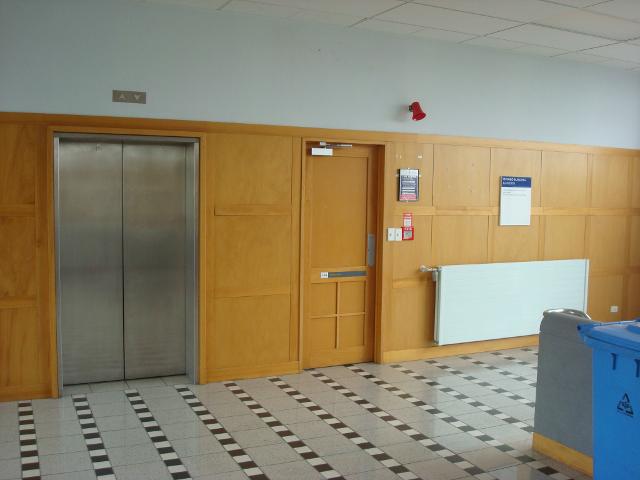
\includegraphics[width=\textwidth]{images/indoor.png}
                \caption{Central hall of 3rd floor.}
                \label{fig:sifta}
        \end{subfigure}
        \begin{subfigure}[b]{0.40\textwidth}
                \centering
                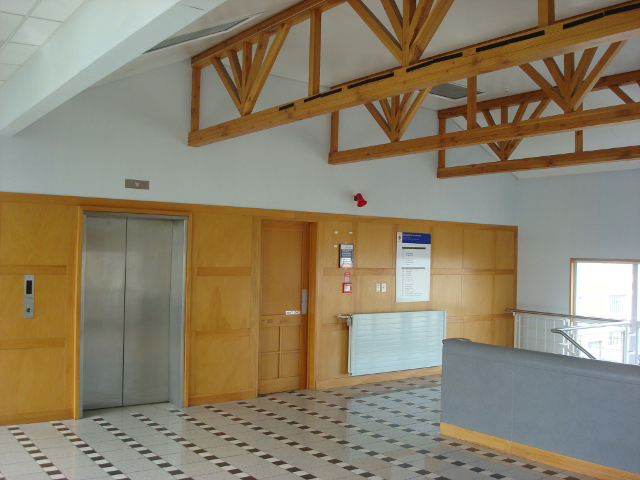
\includegraphics[width=\textwidth]{images/indoor1.png}
                \caption{Central hall of second floor.}
                \label{fig:siftb}
        \end{subfigure}
      \caption{Images of two locations with in the office building with huge similarities.}
 \label{fig:sampleindoor} 
\end{figure}


In order to address the mentioned limitations,
we have proposed an "Indoor Positioning System (iPoS)" which is currently 
based on a client server model and targets the blind users. 
The smartphone application 
allows its user to take a picture of the indoor scene, sends 
it to the server to find the best match and then 
generates a voice message on the smartphone 
to indicate the current location. 
The algorithms which enable iPoS to operate robustly include 
firstly, a proposed visual Bag of Words (BoW) 
scheme for relevant image retrieval. 
Secondly a verification method to verify the location 
match followed by further validation if required.
We have tested our system
in large indoor environments and got good results. 
Our results show that single camera is 
a feasible sensor for indoor positioning 
in real time in challenging indoor environments.

%-------------------------------------------------------------------
\section{Motivation}
\label{sec:motivation}
There are about 11,500 people in New Zealand 
who are either blind or have a low vision (~\cite{rnzfb}).
By 2020, the population of blind people in New Zealand 
is estimated to rise up to 18,300. While population 
of blind people have risen to 39 million all over 
the world lately (~\cite{who12}).
Therefore, a cost effective solution 
is required for the blind people in coming years.

Indoor positioning systems based on non-vision 
sensors such as infrared light (~\cite{roy92}), 
ultrasonic (~\cite{ko08}), Wi-Fi (~\cite{paul08}) 
and Active-RFID (~\cite{ni04}) have been proposed. 
The indoor localisation system based on any sensor 
should at least meet some requirements: (1)
equipment cost should be less, 
(2) positioning accuracy should be high,  
(3) handling of multiuser should be there, 
and (4) easy to use for the blind people.
The performance comparison of different sensors 
keeping in mind the mentioned requirements 
in summarized in Table \ref{tab:tech} (~\cite{kawaji10}). 
The image processing or vision solutions based 
on a mobile camera seem to offer 
a cost effective solution with reasonable accuracy. 
Therefore, the main motivation our research work is to:

\emph{
\begin{quote}
come up with a robust localization system based solely on vision 
which is easy to use and can provide rough guidance 
to blind people during navigation 
in office and non-office buildings. 
\end{quote}
}
\begin{table}

\caption{Performance comparison of existing technologies}
\centering
\begin{tabular}{|c|c|c|}
\hline 
Technology & Positioning accuracy & Equipment cost\tabularnewline
\hline
\hline 
Infrared light  & 5-10m  & High \tabularnewline
\hline 
Ultrasonic  & 1-10cm  & High \tabularnewline
\hline 
RFID  & 5cm-5m  & High \tabularnewline
\hline 
Wi-Fi  & 2-100m  & Low-High \tabularnewline
\hline 
Audible sound  & 5-10m  & Middle \tabularnewline
\hline 
Mobile camera & 1-5m  & Low \tabularnewline
\hline
\end{tabular}
\label{tab:tech}
\end{table}




The other motivators for our work are:-

\begin{itemize}
\item Most vision based localization works 
focus  on outdoor environments. 

\item The literature shows not much work 
is done in large scale indoor environments 
using vision. Most works limit experiments 
to few indoor places. 

\item Localisation is often performed 
in context of non office buildings. The 
positioning becomes a challenge in office 
buildings where places are pretty similar. 
Therefore, a localisation system performance 
needs to be analysed in office environment.

\item Video stream is used as an input 
for the real time localization and mapping 
in many works (~\cite{gemeiner08}). 
This is not ideal for blind people
because video stream will drain the 
phone battery and will require 
often charging of the phone. This will 
only add more to the worries of 
blind people.

\item The localization module is often embedded 
in the navigation systems and is not available 
as a separate independent unit.
\end{itemize}



Blind people carry smart phones for making calls, 
reading emails etc and are familiar with most of 
the functionality. The majority of the smartphones 
has a reasonable camera and a 
smartphone application based on vision 
will be really handy 
for the blind people. Blind people can use the 
application when they feel they are lost 
while navigating in indoor buildings. 

%-------------------------------------------------------------------
\section{Challenges and contributions}
\label{sec:contributions}
Most of the successful scene recognition work is 
done in outdoor environments. 
Comparatively, less work is done for office indoor buildings.
It's quite hard to find a framework in which smartphone 
uses a single image of the current scene and 
performs a robust localization. Amongst, the challenges 
we faced were:-

\begin{itemize}

\item Identifying the reliable features
which are capable of good image matching 
with different transformations 
in any environment. 


\item People propose and use different techniques to verify 
the images retrieved from visual BoW but 
on different data sets. 
So there is no standard way for
images verification. 

\item The absence of office building data sets 
for the experimental purposes. 

\item Designing a user friendly interface 
for our smartphone application to 
ptovide maximum accessibility to the 
blind uers.


\item Understanding the camera model coordinate 
systems and transformations 
between 2D features (query image) 
and 3D models (points) for effective pose estimation.

\end{itemize}

We followed a bottom up approach. We first identified the 
best features to be used for image matching 
in our work. We then started with the 
image matching in outdoor environment 
followed by the experiments in our indoor data set. 
After a careful analysis, we proposed a 
robust image matching system which 
can localize the current scene. Finally, we 
developed the smartphone application to send 
the query pictures to our system (running on a 
server) and evaluated the localisation performance 
on real indoor data sets. 
Our main contributions are:-


\begin{itemize}
\item We propose a shorter version of scale invariant feature 
transform (SIFT) features (~\cite{khan12b}) 
for the image matching and compare it with other well known feature 
descriptors.

\item We evaluate the performance of our 
shorter SIFT features thoroughly against 
different image transformations (~\cite{khan11b}). 

\item We evaluate different ranking functions 
namely normalized term frequency ($ntf$), normalized term 
frequency inverse document frequency ($ntfidf$) and 
Okapi $BM25$ for the visual BoW for the analysis. 

\item We compare soft and hard 
assignments schemes  in visual BoW 
for the indoor environment (~\cite{khan11a}). 


\item We propose a visual BoW based on 
a voting module and a verification method. Voting module 
is not only efficient but also effective.


\item We compare different verification methods 
with our proposed homography method for the analysis (~\cite{khan11a}).
Our proposed homography verification method 
gives comparable performance to the fundamental 
matrix based verification and is also efficient. 

\item We propose a track based approach to 
effectively reduce the features from large scale data sets 
up to a 50\%~\cite{khan12c}.


\item We develop a working android application (~\cite{khan12a}). 
The application is refined over time 
in functionality and thoroughly tested on various 
indoor data sets. The current application offers the 
simplest interface which is suitable for blind users (~\cite{khan12b}). 


\item We compare the localisaiton performance 
based on pose estimation and 2D image matching 
with different mobile devices for analysis.
We also propose a hybrid algorithm 
for an effective indoor image matching 
with almost zero wrong matches. 

\item We develop five indoor data sets which 
can be used as a standard to test the classification 
performance in indoor. 
\end{itemize}


%-------------------------------------------------------------------
\section{Application}
\label{sec:applications}

Our system is intended to assist the blind people 
whilst they navigate in indoor buildings. However, 
it is also applicable to other users:-

\begin{enumerate}
\item \textbf{Prospective Students :}
It's hard to figure out the different places 
in the campus in the beginning. Our application 
can offer a natural way of learning information about
the campus by taking pictures and getting pop up 
text messages. The new students can utilize 
this application to get familiar 
with the campus environment. 

\item \textbf{Large malls: } 
It's easy to get lost in 
large shopping malls. This application could help 
shoppers to find where they are and where they want to go.


\item \textbf{Tourists: } 
Each city has a history reflected by the historic landmarks 
(e.g. buildings, statues, historic trees etc).
Our application can serve a guide for tourists, giving 
information about the captured landmark images 
from the smartphone therefore promoting the tourism.

\end{enumerate}


%---------------------------------------------------------------------
\section{Limit of scope}
\label{sec:limitofscope}
In simple scenario, the system takes the 
picture of the current scene and identifies the 
current location. In real time, there are different 
factors which can affect the performance of 
such system. It's is not possible to address all 
challenges in a single PhD project. The limitations of our work 
are:-

\begin{enumerate}
\item The initial target of our work 
was a complete navigation system for 
blind people but  we ended up with localization
due to time constraint. We also did not 
get time to integrate our localisation 
module with any existing navigation system for further 
analysis. 

\item We have not tested our system with blind 
users so far. However, the application may need to 
be voice powered (to launch/ close the application) 
to make it more accessible.

\item We use a non- incremental approach 
and the mapped images of the building are not 
updated whilst application performs localisaiton. 
The system does well with smaller changes with in the indoor 
places as shown in Figure \ref{fig:changes}. 
The maps will need updation 
if major changes happen in 
indoor places. This motivates the use 
of incremental approach to update the trained 
images during navigation (~\cite{angeli08}).
 
\begin{figure}[h!]
\centering
        \begin{subfigure}[b]{0.40\textwidth}
                \centering
                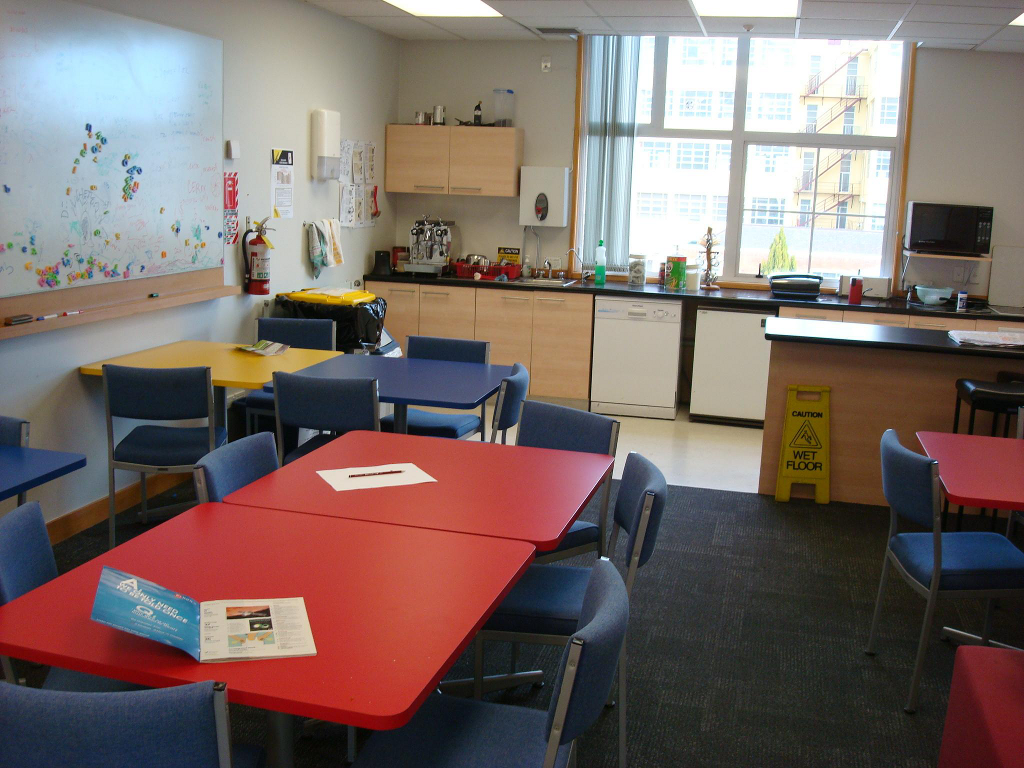
\includegraphics[width=\textwidth]{images/cr_1.png}
                \caption{Trained Image.}
        \end{subfigure}
        \begin{subfigure}[b]{0.40\textwidth}
                \centering
                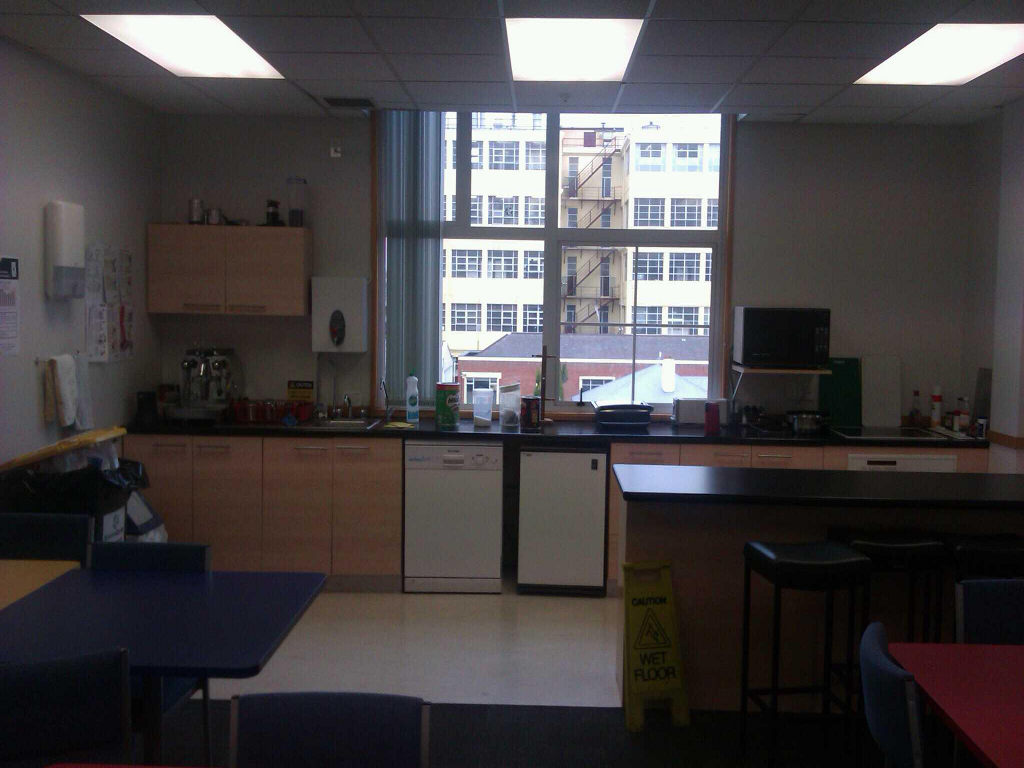
\includegraphics[width=\textwidth]{images/cr_2.png}
                \caption{Query Image.}
        \end{subfigure}
      \caption{Images of the same locations taken after some time.}
 \label{fig:changes} 
\end{figure}


\item Our system works well with a couple of people in the scene 
as shown in Figure \ref{fig:crowd}. The system capability to 
handle more people or crowd is not 
tested and is not the focus of our work.
 
\begin{figure}[h!]
	\centering
                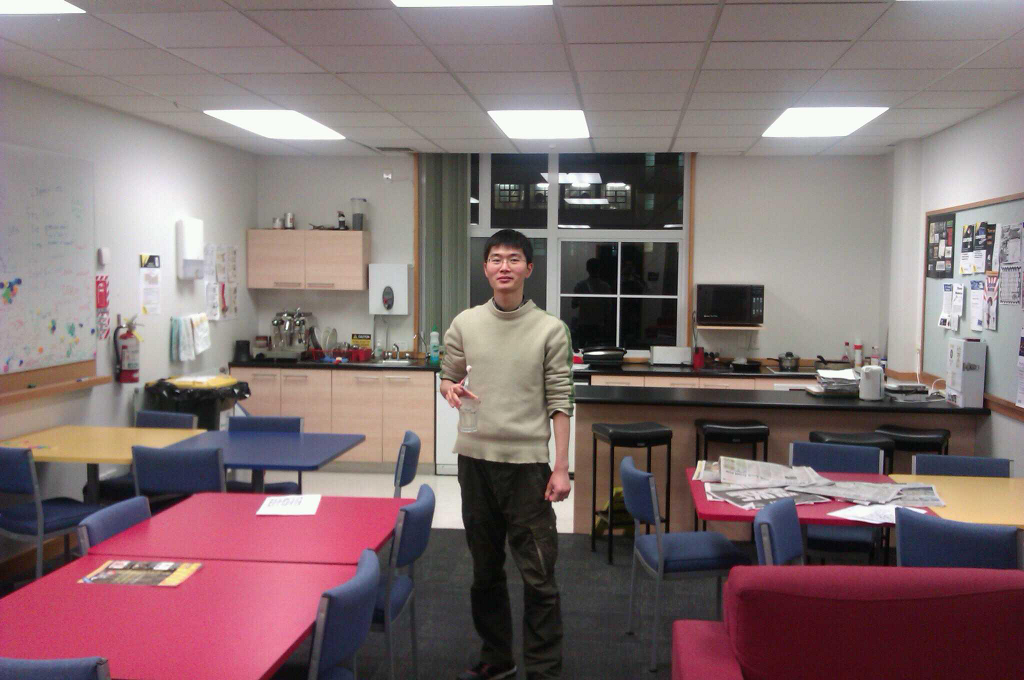
\includegraphics[width=0.4\textwidth]{images/crowd.png}
	      \caption{Query image taken at night.}
 \label{fig:crowd} 
\end{figure}


\item Our vision based localization system 
currently runs on the server. The smartphone 
application is just an interface for sending pictures 
and getting location information. We use 
this configuration for simplicity but 
whole system can be deployed on the smartphone. 



\item The mapped images of the building 
intended for navigation must be 
be labeled. We have developed "Map builder" 
module which needs an excel file filled from the user 
to generate the labels. The automatic labeling 
can also be done by using scene semantics 
or by image classification (~\cite{rasiwasia08, ranga10})
and is not the focus of our work.

\end{enumerate}

%----------------------------------------------------------
\section{Thesis Layout}
\label{sec:overview}

This thesis describes the development of iPoS. 
To achieve this, the used algorithms and corresponding evaluations 
on data sets are discussed in the chapters one by one. 
This thesis consists of nine chapters and details are 
as follows:-

\begin{enumerate}
\item \textbf{Chapter 2} gives an overview about 
navigation system requirements in context 
of blind users and presents some navigation 
tools which are in use of blind people.

\item \textbf{Chapter 3} presents research works 
which perform vision based indoor navigaiton 
and can guide the blind people. The localisation 
importance in visual navigation is further discussed followed 
by overview of some techniques used for indoor and 
outdoor scene recognition. 

\item \textbf{Chapter 4} states all data sets 
and metrics used in this thesis for performance 
evaluation. 

\item \textbf{Chapter 5} proposes a shorter versions of SIFT 
feature descriptor and compares it 
with different feature descriptors 
for general image matching on different data sets.

 \item \textbf{Chapter 6} proposes a visual Bag of Words (BoW) 
approach based on the shorter features proposed 
in Chapter 5. The proposed system is compared with 
a normal system with different configurations for 
performance analysis.

\item \textbf{Chapter 7} is a comparison 
of different verification methods 
which can be used with our proposed BoW presented 
in Chapter 6.

\item \textbf{Chapter 8} presents ways to reduce the 
features proposed in Chapter 4. The target 
was to use reduced features with proposed BoW 
for more robust image matching.

\item \textbf{Chapter 9} is evaluation of image localisation 
using pose estimation and simple 2D image matching 
with different mobile devices for the analysis. 

\item \textbf{Chapter 10} presents the framework 
used by us for the smartphone application. 
The system performance in real time data sets 
are reported in this chapter.

\item \textbf{Chapter 11} contains the final remarks 
and suggestions for possible future research work. 

\end{enumerate}

%----------------------------------------------------------
\section{Publications}
\label{sec:publicatios}

\begin{enumerate}
\item (~\cite{khan11a}) Proceedings of Image and Vision Computing New Zealand. 
This paper presents a proposed visual BoW 
based on voting scheme and homography method for a 
robust image matching.

\item (~\cite{khan11b})  Proceedings of International 
Conference on Digital Image Computing: 
Techniques and Applications (Australia). This paper discusses the proposed 
shorter version of SIFT features and compare it with SURF.

\item (~\cite{khan12a}) Proceedings of International 
Conference of the NZ Chapter of the 
ACM's Special Interest Group on Human-Computer Interaction. 
We discuss the first prototype of our smart phone application 
and reported the preliminary results. 

\item (~\cite{khan12b}) Proceedings of 14th International 
ACM SIGACCESS conference on Computers and Accessibility (USA).
We present the final prototype of our system 
and test it on larger images. 


\item  (~\cite{khan12c}) 
Proceedings of Image and Vision Computing New Zealand.
We propose the method to reduce the features from 
trained images by more than 50\% and compare 
our reduced features against well known descriptors.

\end{enumerate}
\subsection{APPSTAR Competition}
APPSTAR was a competition run by Otago Innovation Ltd, Otago University in 
2012. The competition asked the University of Otago’s academic and research 
staff and students all over the New Zealand 
to put forward an idea for a mobile or web Application. 
The competition received an incredible 108 entries and 
5 ideas were selected by a panel of Judges.
Our application in collaboration with William Levack 
'Living it up/iPos" was one of the top 5 finalists in the competition. 
The basic theme of 'Living it up/iPos" was 
to help people with memory loss to know exactly 
where they are in their house and then 
guide them to perform daily life time activities. 
For example if someone is in the kitchen 
then he/she can be prompted with a 
list of things to do such as make a breakfast, 
cooking tips etc.
 

